\begin{figure}
    \centering
    \begin{tabular}{>{\centering\arraybackslash}p{0.42\textwidth}>{\centering\arraybackslash}p{0.42\textwidth}}
    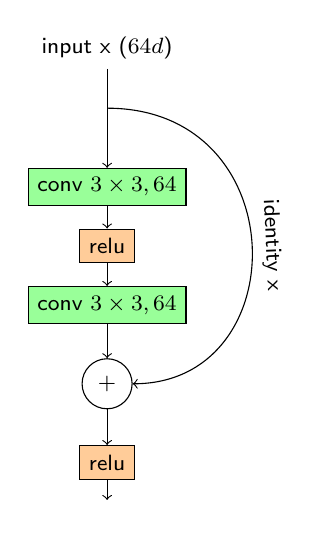
\begin{tikzpicture}[font=\footnotesize\sffamily]
        \path (0, 5) node[above](xinp) {input x ($64d$)}
              (0, 3.5) node[fill=green!40, draw](xc1) {\gls{conv} $3\times3, 64$}
              (0, 2.75) node[fill=orange!40, draw](xr1) {\gls{relu}}
              (0, 2) node[fill=green!40, draw](xc2) {\gls{conv} $3\times3, 64$}
              (0, 1) node[circle,draw](xplus) {+}
              (0, 0) node[fill=orange!40, draw](xend) {\gls{relu}}
              (0, -0.6) node(xout) {};
        \draw[->] (xinp) -- (xc1);
        \draw[->] (xc1) -- (xr1);
        \draw[->] (xr1) -- (xc2);
        \draw[->] (0, 4.5) .. controls +(right:2.4cm) and +(right:2.4cm) .. node[sloped, above] {identity x} (xplus);
        \draw[->] (xc2) -- (xplus);
        \draw[->] (xplus) -- (xend);
        \draw[->] (xend) -- (xout);
    \end{tikzpicture} &

    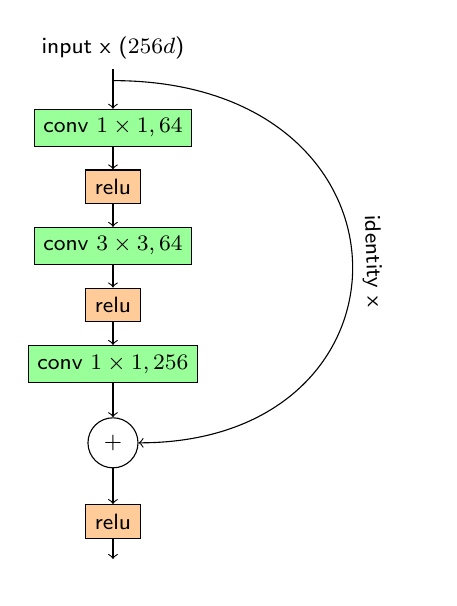
\begin{tikzpicture}[font=\footnotesize\sffamily]
        \path (0, 5.75) node[above](xinp) {input x ($256d$)}
              (0, 5) node[fill=green!40, draw](xc1) {\gls{conv} $1\times1, 64$}
              (0, 4.25) node[fill=orange!40, draw](xr1) {\gls{relu}}
              (0, 3.5) node[fill=green!40, draw](xc2) {\gls{conv} $3\times3, 64$}
              (0, 2.75) node[fill=orange!40, draw](xr2) {\gls{relu}}
              (0, 2) node[fill=green!40, draw](xc3) {\gls{conv} $1\times1, 256$}
              (0, 1) node[circle,draw](xplus) {+}
              (0, 0) node[fill=orange!40, draw](xend) {\gls{relu}}
              (0, -0.6) node(xout) {};
        \draw[->] (xinp) -- (xc1);
        \draw[->] (xc1) -- (xr1);
        \draw[->] (xr1) -- (xc2);
        \draw[->] (xc2) -- (xr2);
        \draw[->] (xr2) -- (xc3);
        \draw[->] (0, 5.6) .. controls +(right:4cm) and +(right:4cm) .. node[sloped, above] {identity x} (xplus);
        \draw[->] (xc3) -- (xplus);
        \draw[->] (xplus) -- (xend);
        \draw[->] (xend) -- (xout);
    \end{tikzpicture}
    \\[6pt]
    (a) A simple non-linear residual block. & (b) A bottleneck block as employed in the deeper \glspl{resnet}.
    \end{tabular}

    \caption{Two examples of residual blocks. The input of the block is fused into the ouptut of the last \gls{conv} layer and added element-wise channel-per-channel onto it. A \gls{relu} is trailing the sum again.}
    \label{fig:resblock}
\end{figure}
